
This Section introduces use cases and the specified Quality Attribute Scenarios (QAS).
The QASs are developed based on the use case.

\subsection{Use case}
\label{sec:use_case}
After going through the system requirements and quality attributes, our team delved into an analysis of the end user's factory. Drawing on insights from related works, we crafted a set of use cases that thoroughly cover all the essential functionalities needed for the end user's factory.

Most of the use cases are detailed in the appendix (see \ref{sec:apusecase}), with a focus on the most pivotal one outlined below:

\vspace{1em}
\begin{itemize}
    \item \textbf{Use Case Name:} User Orders a Tank
    \item \textbf{Actors:} User, Order Creator, Scheduler
    \item \textbf{Preconditions:} The user is on the website and has decided on the type of tank they want.
    \item \textbf{Steps:}
    \begin{itemize}[label=--]
        \item User creates an order for tank(s).
        \item The order is saved to a database.
        \item The order creator reads the database and sends it to the scheduler.
        \item The scheduler processes the order for the related components and responds to the order creator which it received the order from and begins to process it.
        \item Order creator updates the status of the order in the database.
        \item The website shows the updated status to the user.
    \end{itemize}
    \item \textbf{Postconditions:} An order has been scheduled, and all affected components are notified.
\end{itemize}
\vspace{1em}

The highlighted use case centers on the primary system flow, illustrating how a user places an order for a tank. The key actors in this scenario are the User, Order Creator, and Schedulers. The User, representing the individual or company placing the order, interacts with a subsystem comprised of the Order Creator and Schedulers. More details on their responsibilities and design can be found in Section \ref{sec:middleware_architecture}.

The sequential steps delineate the user journey through the interface, outlining the process of ordering a tank. Notably, the user interface deliberately avoids direct communication with the schedulers to minimize coupling.

Upon placing an order, the system stores the order information in a database. Subsequently, a dedicated subsystem reads the order from the database and forwards it to the schedulers. This intentional decoupling ensures that the interoperability of the system is maximized, thereby enhancing overall flexibility and adaptability.

This use case provides a detailed examination of how the system leverages multiple smaller subsystems to seamlessly deliver a cohesive whole. 
This is demonstrated through the various actors and the postconditions statement that outlines the impact on the rest of the affected components. This connection ties the use case to quality attributes (QA) interoperability across the subsystems. The use case also encapsulates QA for availability, as a system failure of components like the Scheduler would impede the user's functionality.

Furthermore, additional use cases underline the significance of component architecture. Extensive research has highlighted the advantages of adopting a microservice architecture for its scalability and interoperability. Designing and deploying a system becomes considerably more straightforward when anchored in such an architecture.

\subsection{Quality attribute scenarios}
\label{sec:qas}
After developing the use cases, the team proceeded to create quality attribute scenarios for various attributes, including performance, scalability, deployability, and availability. The selection of these attributes was formulated based on the research from related works and the use cases that was developed.

In particular, we have chosen to showcase the QAS for availability as this will be the primary focus of testing in the Evaluation section (see Section \ref{sec:evaluation}).

The featured use case revolves around the user's tank order process, directly impacting the QAS in focus. The availability of the tank-manufacturing robot is critical, as the order cannot progress without it. Therefore, ensuring the prompt processing of tank orders is heavily dependent on the immediate availability of the manufacturing robot once the order has been configured. 


\begin{center}
    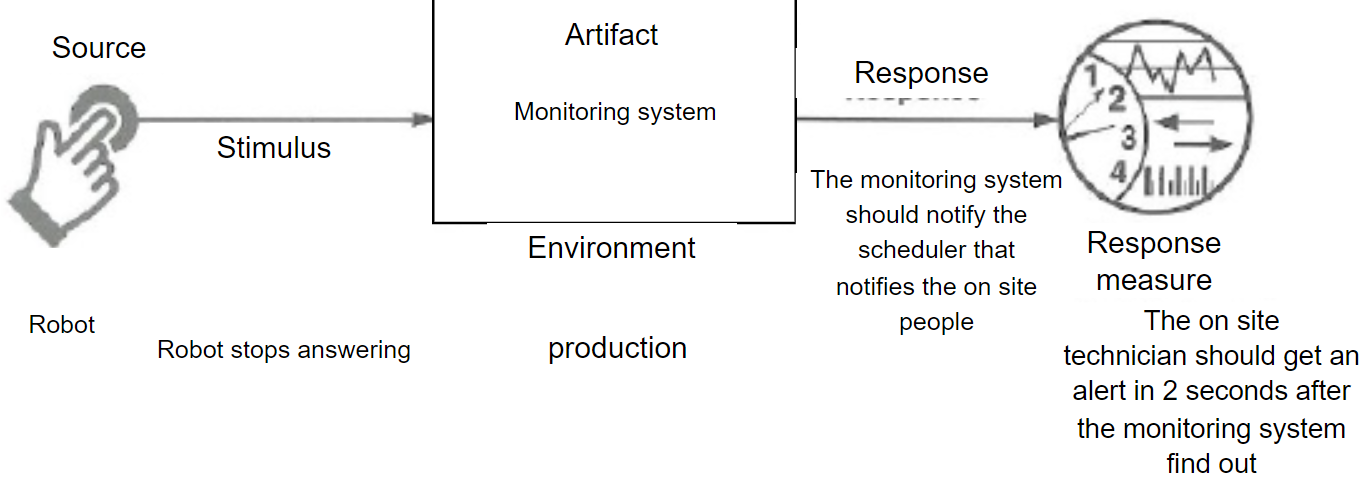
\includegraphics[scale= 0.26]{Images/availability.png}
\end{center}
In the appendix there is a bigger version and also the rest of the QASs (see \ref{sec:QAS}).
To showcase the availability scenario each step of it will be explained:
\begin{itemize}
    \item \textbf{Source} Robot
    \item[-]This Scenario is about a given robot in the factory 
    \item \textbf{Stimulus} Robot stops answering
    \item[-] The scenario begins when a robot stops communicating with the monitoring system, detected by the heartbeat system.
    \item \textbf{Artifact} Monitoring System
    \item[-] The artifact is a monitoring system that acts on this stimulus
    \item \textbf{Environment} Production
    \item[-] The environment is a normal production since this scenario could happen at any time in production
    \item \textbf{Response} The monitoring system should notify the scheduler, which then notifies the people on site
    \item[-] The appropriate response from the monitoring system is to notify the scheduler, which will then notify the responsible repair crew in the factory.
    \item \textbf{Response measure} The on-site technician should get an alert in 2 seconds after the monitoring system registers an issue.
    \item[-] The Response measure is equal to how fast the repair crew is notified. 
\end{itemize}
So after the repair crew has either repaired or changed the robot the system should be notified, and the user in the use case should get an notification that the order is beginning production.

All other Quality Attribute Scenarios (QASs) were systematically developed using a similar coupling to specific use cases. This deliberate approach was taken to ensure the relevance of each QAS to the overall system. Additionally, each QAS was associated with a distinct artifact to guarantee that the scenarios encompassed the entirety of the system. This methodology was implemented to prevent a singular focus on a particular aspect of the system during the development of use cases and QAS, promoting a holistic understanding of system performance and behavior.
